\section{PostgreSQL}
PostgreSQL is an ORDBMS - abbreviation for open source object-relational database management system. Origins date back to the year 1986, where the project then known as POSTGRES started as a reference to the older INGRES database. One decade later it got renamed to PostgreSQL to clearly show its ability to work with SQL.\cite{PostgreSQL} 

Nowadays, it's widely used. PostgreSQL popularity has been steadily rising in the last few years. Based on "Stack Overflow Annual Developer Survey"~\cite{Stackoverflow survey}, PostgreSQL currently sits in second place for the 'Most popular technology in the database category', right after the MySQL.

\subsection{Parse tree}
Postgres internally uses parse trees to process SQL Queries. The whole parsing comprises multiple stages. First, a query passed in form of plain text is transformed to tokens using a tool "Flex". Next up the parser generator called "Bison" is called, which consists of multiple grammar rules and actions. Each action is executed whenever any of the rules are applied and together they are used to build the final parse tree.
\newline

\begin{figure}[h]
  \makebox[\textwidth]{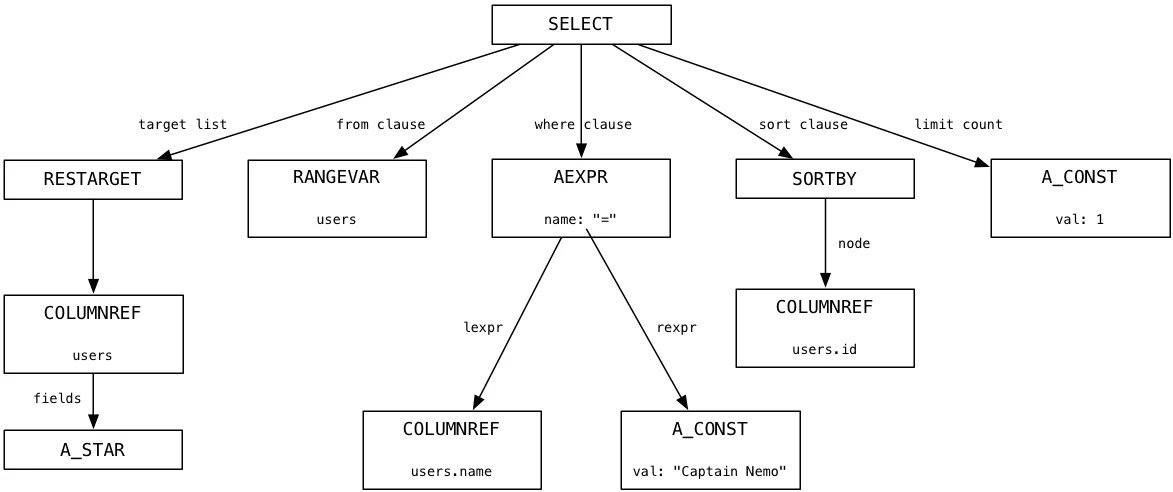
\includegraphics[width=\textwidth]{parse_tree.jpg}}
  \caption {Visualisation of parse tree for \texttt{"SELECT * FROM users WHERE name = 'Captain Nemo' ORDER BY id ASC LIMIT 1"}}
\end{figure}